% Figure from MATH 493 notes, section 56 (stitching two composition series through N: the island and the bridge). Added, not from lecture (after the lecture's image).
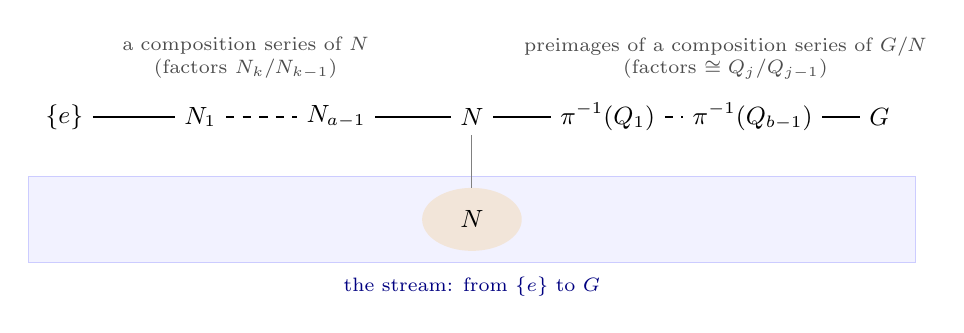
\begin{tikzpicture}[font=\small, >=stealth, x=1.15cm]
  \draw[blue!20, fill=blue!5] (-0.4,-0.55) rectangle (9.4,0.55);
  \node[blue!50!black, font=\scriptsize] at (4.5,-0.85) {the stream: from $\{e\}$ to $G$};
  \fill[brown!20] (4.5,0) ellipse (0.55 and 0.4); \node at (4.5,0) {$N$};
  \node (a0) at (0,1.3) {$\{e\}$}; \node (a1) at (1.5,1.3) {$N_1$}; \node (a2) at (3,1.3) {$N_{a-1}$};
  \node (b0) at (6,1.3) {$\pi^{-1}(Q_1)$}; \node (b1) at (7.6,1.3) {$\pi^{-1}(Q_{b-1})$}; \node (b2) at (9,1.3) {$G$};
  \node (nn) at (4.5,1.3) {$N$};
  \draw[thick] (a0) -- (a1); \draw[thick, dashed] (a1) -- (a2); \draw[thick] (a2) -- (nn); \draw[thick] (nn) -- (b0); \draw[thick, dashed] (b0) -- (b1); \draw[thick] (b1) -- (b2);
  \draw[gray] (4.5,0.4) -- (nn.south);
  \node[font=\scriptsize, align=center, text=black!70] at (2,2.05) {a composition series of $N$\\ (factors $N_k/N_{k-1}$)};
  \node[font=\scriptsize, align=center, text=black!70] at (7.3,2.05) {preimages of a composition series of $G/N$\\ (factors $\cong Q_j/Q_{j-1}$)};
\end{tikzpicture}
